\section{Modellering af Psykolog Nord og deres problemstilling}

Nu da der er en dybere forståelse for Psykolog Nord, deres problem og deres krav til løsningen, kan der kigges nærmere på, hvordan dette projekt har forsøgt at løse deres problemer.
Inden der skrives en masse kode er det dog nødvendigt at arbejde med deres problem og få det omdannet til modeller, som er nemmere at skrive et program ud fra.
Dette vil der blive arbejdet med i dette kapitel.

\subsection{Objektmodel}

For at have et værktøj til at skabe et overblik over virksomheden og dens gøremål, har vi lavet en objektmodel.
Modellen er lavet ud fra møderne med Psykolog Nord, og viden tilegnet sig virksomheden gennem deres hjemmeside.\cite{psykolognord}

Objektmodellen, der kan ses på figur \ref{system:objekt} er udarbejdet med henblik på use casen ``Book Aftale'' beskrevet i afsnit \ref{usecase:bookaftale}.

Vi bruger objektmodellen til at hjælpe os med at visualisere hvilke ting fra Psykolog Nords hverdag, som vi skal have vores system til at indeholde.
Det er også et godt værktøj til at vise Psykolog Nord vores forståelse af deres arbejdsgang og virkelighed.

Objektmodellen er blevet opdateret hele vejen igennem forløbet, og den har været diskuteret igennem med vejledere og alle gruppens medlemmer flere gange.

Vores klientobjekt indeholder blandt andet et informationspunkt, der hedder journal.
Det har været diskuteret meget frem og tilbage i projektgruppen, om det skulle være sit ejet objekt eller ej.
Et argument for at have journalen som sit eget objekt vil være, at informationen i journalen bliver ændret uden at resten af klientobjektet ændres.
Vi har valgt at have det som et informationspunkt, da der altid vil være en en-til-en sammenhæng mellem en klient og en journal, og når en klient bliver oprettet, skal den også have en journal.

\begin{sidewaysfigure}
    \caption{Objektmodel for Book Aftale}
    \centering
        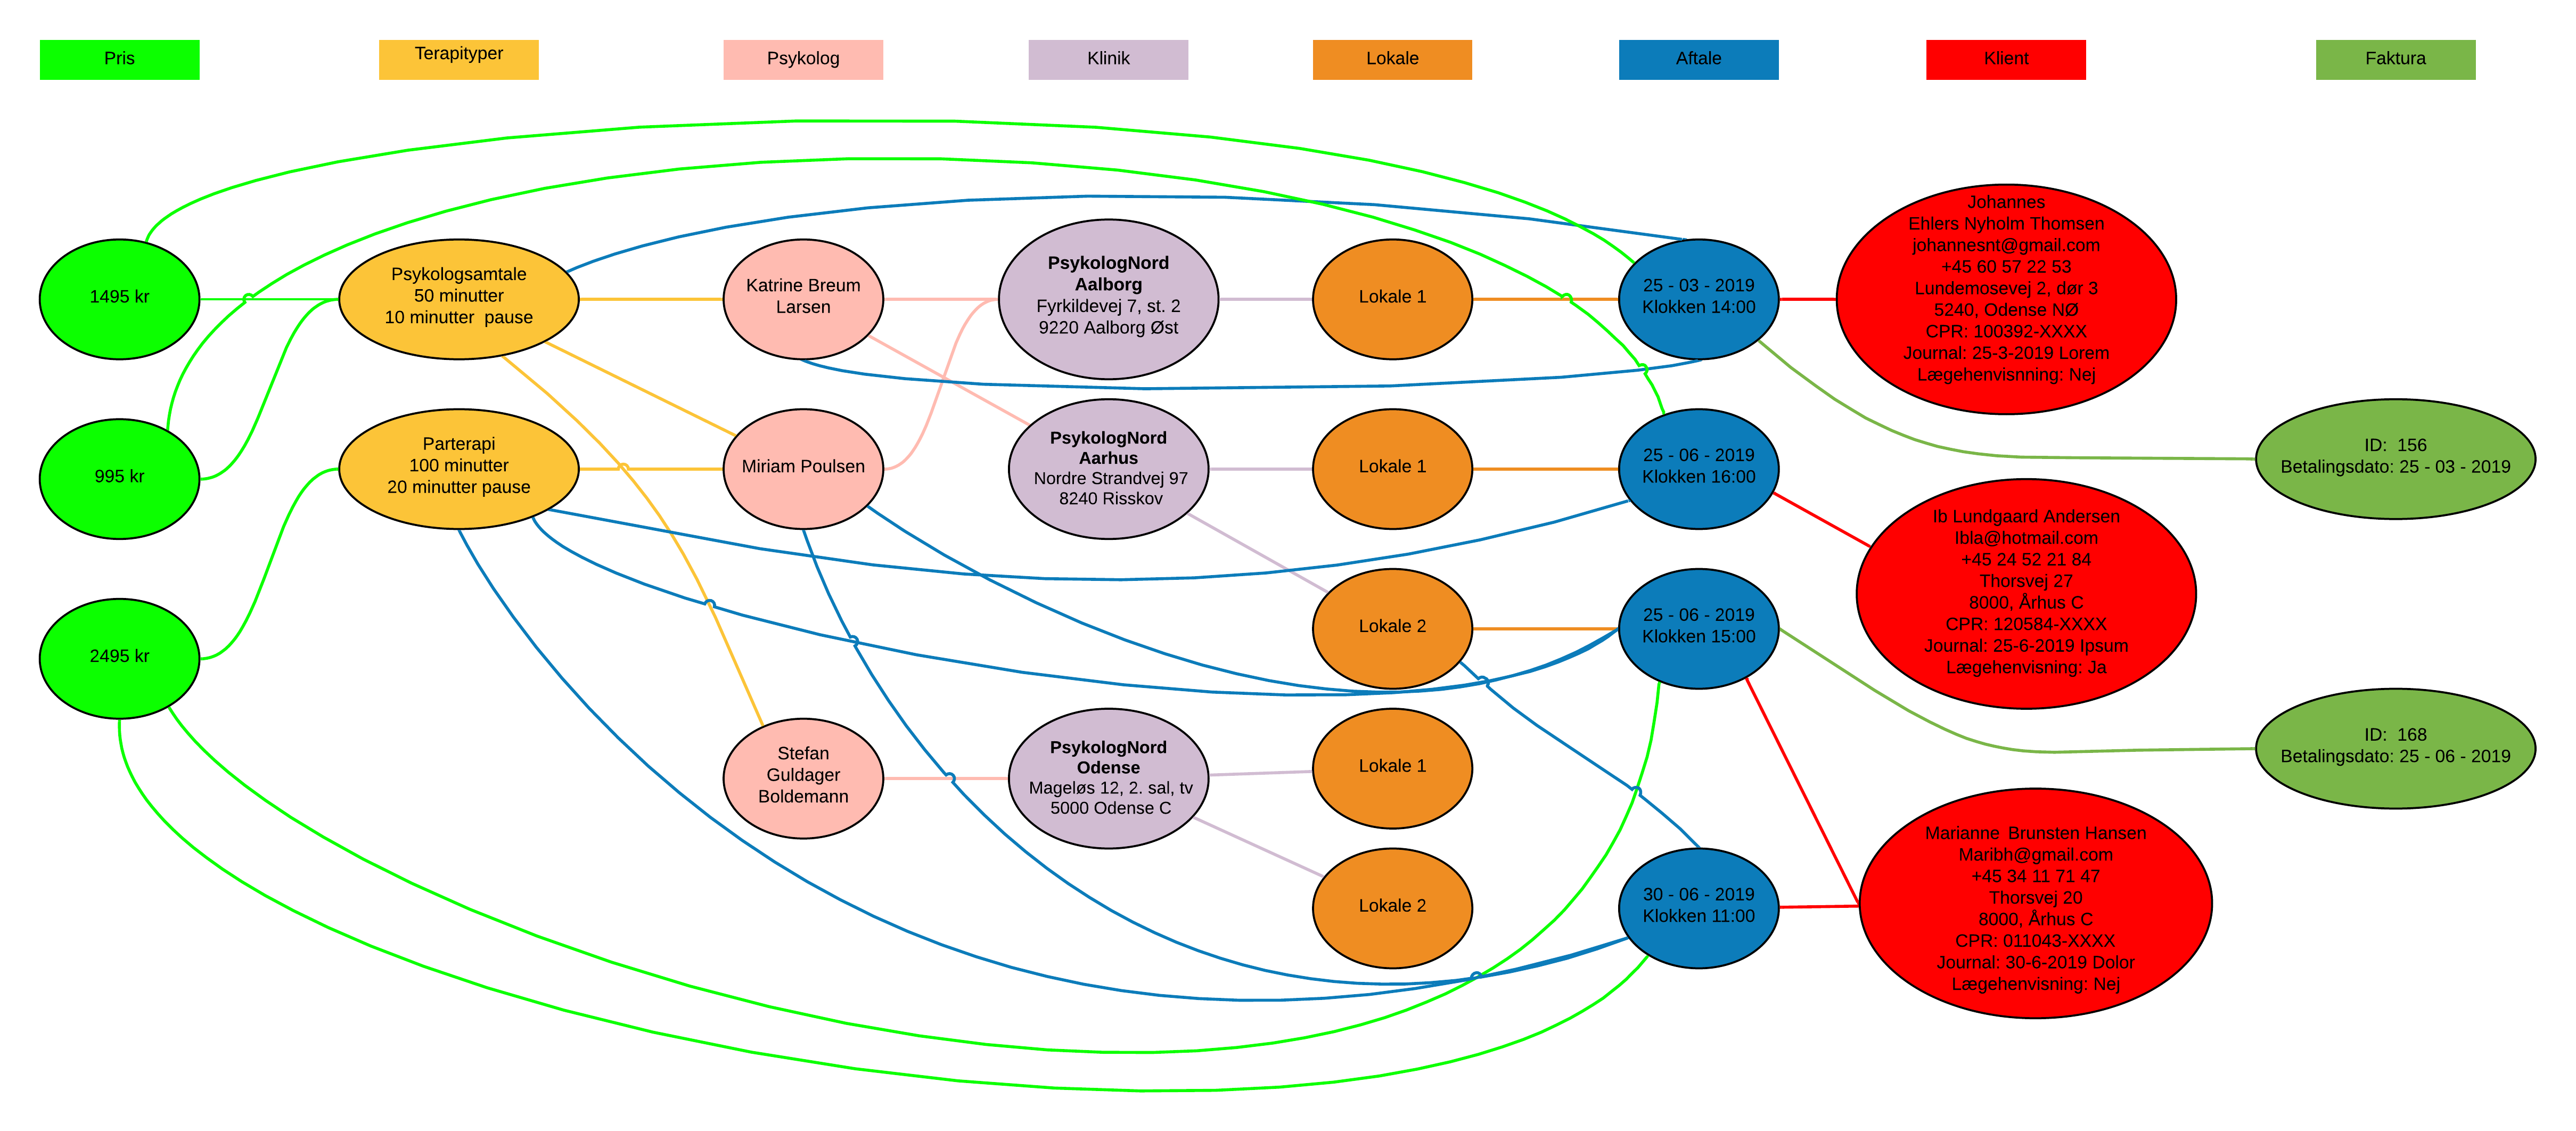
\includegraphics[width=\textwidth]{Objektmodel.png}
    \label{system:objekt}
\end{sidewaysfigure}

